\hypertarget{_p_i_chargedparticles_PI_chargedparticles_main}{}\section{The source file (main.\+cpp)}\label{_p_i_chargedparticles_PI_chargedparticles_main}
The source file is main.\+cpp. This file contains the following code\+: 
\begin{DoxyCodeInclude}
\textcolor{comment}{/* This file is part of PIL, the Particle Interaction Library.}
\textcolor{comment}{ *}
\textcolor{comment}{ * Copyright (C) 2012 by Giacomo Po <gpo@ucla.edu>}
\textcolor{comment}{ * Copyright (C) 2012 by Shao-Ching Huang <sch@ucla.edu>}
\textcolor{comment}{ * Copyright (C) 2012 by Tajendra Singh <tvsingh@ucla.edu>}
\textcolor{comment}{ * Copyright (C) 2012 by Tamer Crosby <tcrosby@ucla.edu>}
\textcolor{comment}{ *}
\textcolor{comment}{ * PIL is distributed without any warranty under the}
\textcolor{comment}{ * GNU General Public License (GPL) v2 <http://www.gnu.org/licenses/>.}
\textcolor{comment}{ */}


\textcolor{preprocessor}{#include <\hyperlink{_terminal_colors_8h}{model/Utilities/TerminalColors.h}>}
\textcolor{preprocessor}{#include <\hyperlink{_sequential_output_file_8h}{model/Utilities/SequentialOutputFile.h}>}

\textcolor{preprocessor}{#include <\hyperlink{_charged_particle_8h}{tutorials/ParticleInteraction/ChargedParticles/ChargedParticle.h}
      >} \textcolor{comment}{// a user-defined type of particle to be inserted in ParticleSystem}
\textcolor{preprocessor}{#include <\hyperlink{_particle_system_8h}{model/ParticleInteraction/ParticleSystem.h}>}

\textcolor{preprocessor}{#include <\hyperlink{_m_p_icout_8h}{model/MPI/MPIcout.h}>}

\textcolor{comment}{//#include <tutorials/ParticleInteraction/ChargedParticles/CoulombEnergy.h> // a user-defined type of
       energy interaction between ChargedParticle objects}



\textcolor{keyword}{using namespace }\hyperlink{namespacemodel}{model};

\textcolor{keywordtype}{int} \hyperlink{bench_2bary_search_2main_8cpp_a0ddf1224851353fc92bfbff6f499fa97}{main} (\textcolor{keywordtype}{int} argc, \textcolor{keywordtype}{char} * argv[]) \{

    \textcolor{comment}{// 0- define the type of ParticleSystem specifying the type of particles}
    \textcolor{keyword}{enum}\{\hyperlink{plot_search_8m_a382f3ca768b275b8d563604f7fc7df73}{dim}=3\}; \textcolor{comment}{// We work in three dimensions}
    \textcolor{keyword}{typedef} \hyperlink{classmodel_1_1_charged_particle}{ChargedParticle<dim>} ChargedParticleType; \textcolor{comment}{// the type of particle}
    \textcolor{keyword}{typedef} \hyperlink{structmodel_1_1_particle_system}{ParticleSystem<ChargedParticleType>} ChargedParticleSystem;
    
    \textcolor{comment}{// 1- create a particleSystem of ChargedParticle(s)}
    ChargedParticleSystem particleSystem(argc,argv); \textcolor{comment}{// initialized constructor: for both serial and
       parallel}
    \textcolor{comment}{//ChargedParticleSystem particleSystem; // uninitialized constructor: for both serial and parallel}
    \textcolor{comment}{//ChargedParticleSystem::initMPI(argc,argv); // if uninitialized constructor is used, call initMPI
       (parallel only)}
    
    \textcolor{keywordtype}{double} cellSize=1.0;
    particleSystem.setCellSize(cellSize);
    
    \textcolor{comment}{// 2- add some ChargedParticle(s) to the particleSystem with random position}
    \textcolor{comment}{//    in [-10,10] and charge=1.0}
    \hyperlink{namespacemodel_a0ce25fef078a7d9d9cb7cfbabcfbc289}{model::cout}<<\textcolor{stringliteral}{"Creating particles..."}<<std::endl;
    \textcolor{keyword}{typedef} \textcolor{keyword}{typename} \hyperlink{classmodel_1_1_charged_particle_a31a77e0315958d087309087da65b422d}{ChargedParticle<dim>::VectorDimD} VectorDimD; \textcolor{comment}{// helper}
    \textcolor{keywordflow}{for} (\textcolor{keywordtype}{size\_t} \hyperlink{run_multipole_8m_a1c73327b2882639bc9f5e416bb3cc7ac}{k}=0;\hyperlink{run_multipole_8m_a1c73327b2882639bc9f5e416bb3cc7ac}{k}<500000;++\hyperlink{run_multipole_8m_a1c73327b2882639bc9f5e416bb3cc7ac}{k})
    \{
        \textcolor{keyword}{const} VectorDimD \hyperlink{plot_nd_a_8m_a2de865ad6dc88c711fbee00e74ed3043}{P}(VectorDimD::Random()*10.0*cellSize); \textcolor{comment}{// PositionType::Random() returns values
       in [-1, 1]}
        \textcolor{keyword}{const} VectorDimD \hyperlink{run_multipole_8m_ac0055fa4cdc19a2690bfee3643413a7d}{V}(VectorDimD::Random()*0.0);
        \textcolor{keyword}{const} \textcolor{keywordtype}{double} q(1.0);
        particleSystem.addParticle(\hyperlink{plot_nd_a_8m_a2de865ad6dc88c711fbee00e74ed3043}{P},\hyperlink{run_multipole_8m_ac0055fa4cdc19a2690bfee3643413a7d}{V},q);
    \}

    \textcolor{comment}{// Add a more particles}
\textcolor{comment}{//    for (int k=0;k<500;++k)}
\textcolor{comment}{//    \{}
\textcolor{comment}{}\textcolor{comment}{//                particleSystem.addParticle(PositionType::Random()*10.0, 1.0); // uniform}
\textcolor{comment}{//    \}}
    
    
    \hyperlink{namespacemodel_a0ce25fef078a7d9d9cb7cfbabcfbc289}{model::cout}<<\textcolor{stringliteral}{"There are "}<<particleSystem.particles().size()
    <<\textcolor{stringliteral}{" particles occupying "}<<particleSystem.cells().size()<<\textcolor{stringliteral}{" cells."}<<std::endl;
    
    \textcolor{comment}{// -3.2a compute all binary CoulombForce interactions}
    \hyperlink{namespacemodel_a0ce25fef078a7d9d9cb7cfbabcfbc289}{model::cout}<<\textcolor{stringliteral}{"Computing electric field (nearest-neighbor)..."}<<std::endl;
    \textcolor{keyword}{typedef} \textcolor{keyword}{typename} ChargedParticleType::Efield Efield;
    particleSystem.computeNeighborField<Efield>();

    \hyperlink{namespacemodel_a0ce25fef078a7d9d9cb7cfbabcfbc289}{model::cout}<<\textcolor{stringliteral}{"Computing magnetic field (nearest-neighbor)..."}<<std::endl;
    \textcolor{keyword}{typedef} \textcolor{keyword}{typename} ChargedParticleType::Bfield Bfield;
    particleSystem.computeNeighborField<Bfield>();

    
    \textcolor{comment}{// -4 output}
    \hyperlink{namespacemodel_a0ce25fef078a7d9d9cb7cfbabcfbc289}{model::cout}<<\textcolor{stringliteral}{"Writing output file P/P\_0.txt..."}<<std::endl;
    \hyperlink{classmodel_1_1_sequential_output_file}{SequentialOutputFile<'P',true>} pFile1;
    pFile1<<particleSystem.particles()<<std::endl;

    
    \textcolor{keywordflow}{return} 0;
\}


\end{DoxyCodeInclude}
\hypertarget{_p_i_chargedparticles_FRsource_makefile}{}\section{Compiling\+: the Makefile}\label{_p_i_chargedparticles_FRsource_makefile}
\begin{DoxyVerb}cd <MODELDIR>/tutorials/ParticleInteraction/ChargedParticles
\end{DoxyVerb}


The same Makefile can now be used to compile both the serial version and the parallel version (M\+P\+I) of the code. The serial version can be compiled executing the following command in your terminal\+: \begin{DoxyVerb}make serial
\end{DoxyVerb}
 This compiles the source code into the executable {\bfseries C\+Pserial}.

Similarly, The parallel version (M\+P\+I) of the code can be compiled using\+: \begin{DoxyVerb}make parallel 
\end{DoxyVerb}
 This creates the executable {\bfseries C\+Pparallel}. Compiling the parallel version requires that both \hyperlink{openmpi}{open-\/\+M\+P\+I} and \hyperlink{metis}{M\+E\+T\+I\+S} are correctly installed in your system.\hypertarget{_p_i_chargedparticles_FRsource_run}{}\section{Running D\+Dserial and D\+Dparallel}\label{_p_i_chargedparticles_FRsource_run}
The serial version of the code can be run executing\+: \begin{DoxyVerb}./CPserial
\end{DoxyVerb}


On the other hand, the parallel version of the code can be run executing\+: \begin{DoxyVerb}mpirun -np N v
\end{DoxyVerb}
 where {\bfseries N} is the number of processors to be used.

 
\begin{DoxyImage}
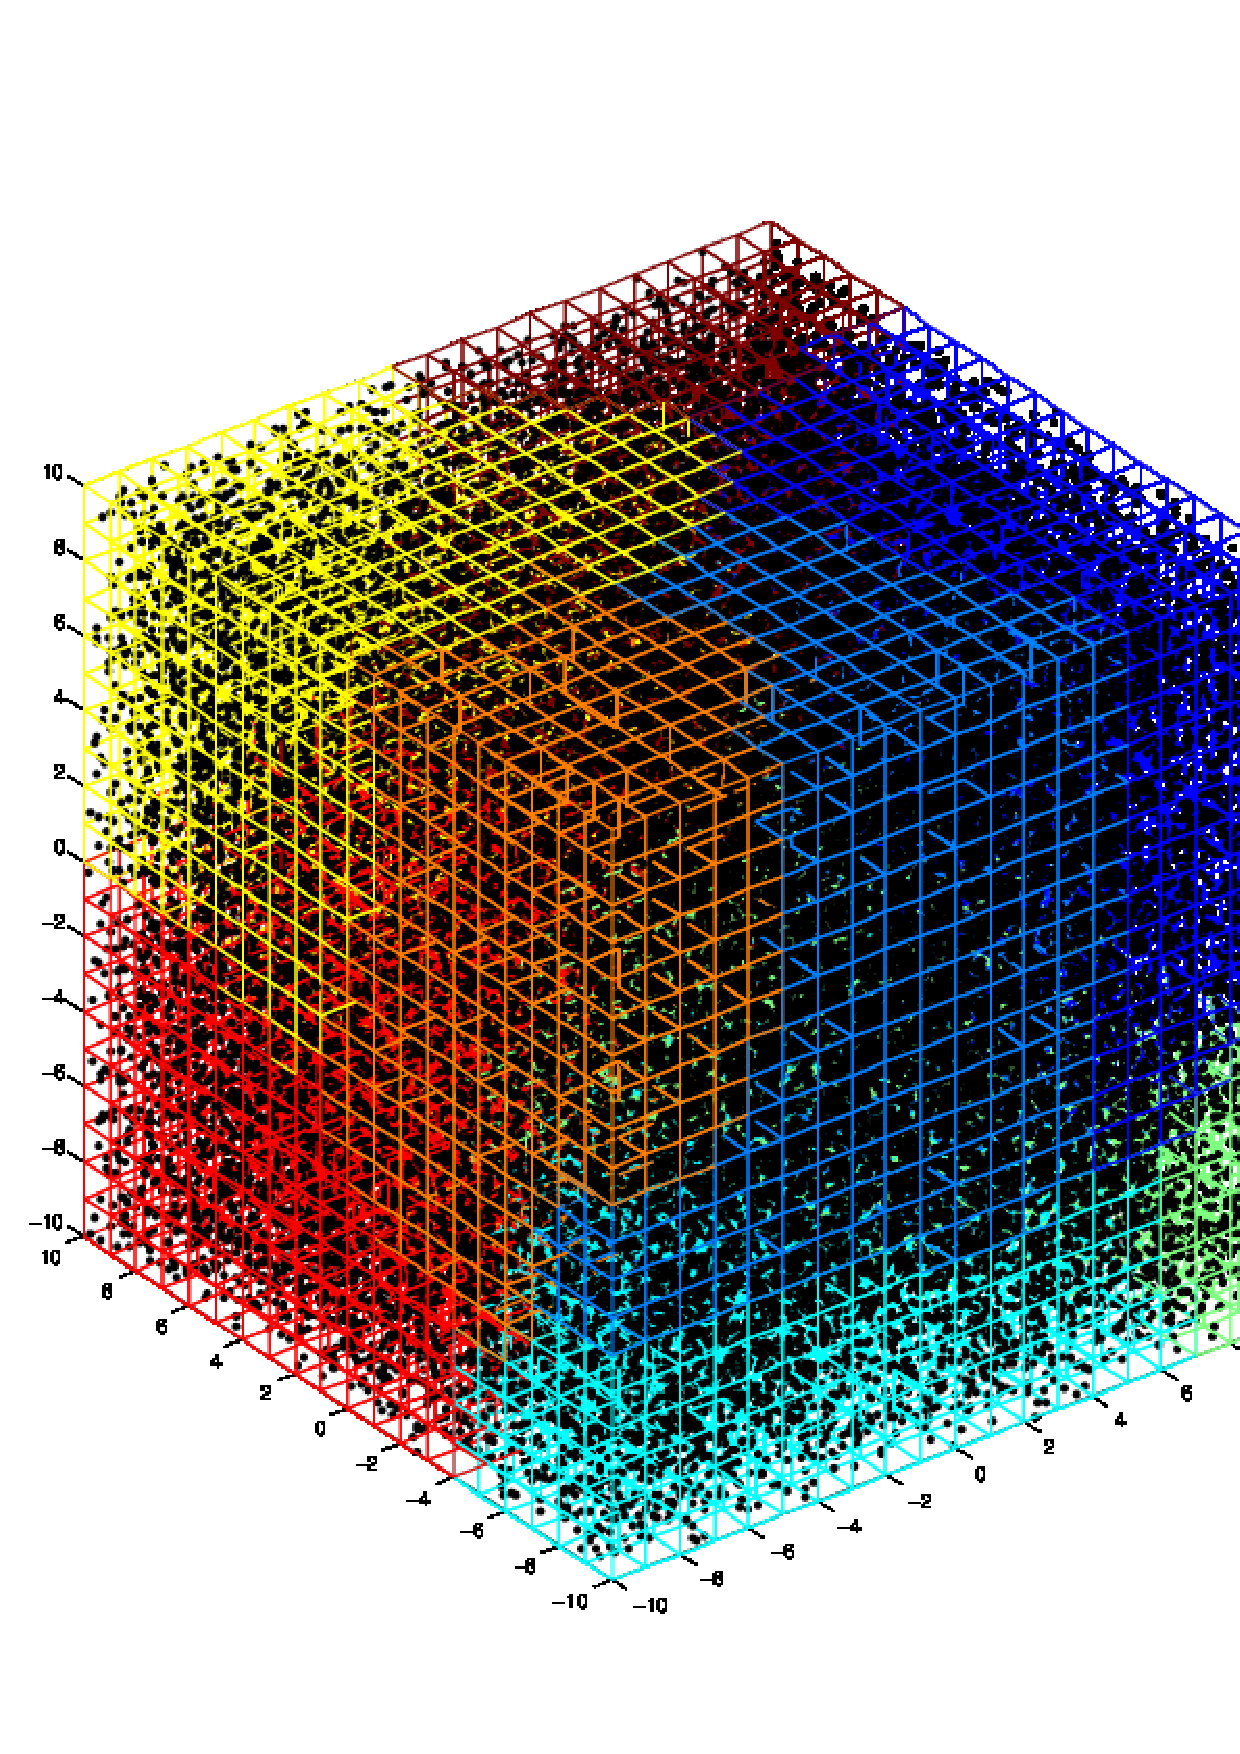
\includegraphics[width=7cm]{cells_50k}
\caption{Decomposition in cells}
\end{DoxyImage}
 